%********************************************************************
% Kapitel 3
%*******************************************************
\chapter{Architecture}
\label{ch:Architecture}

\section{Overview}

In general, the application consists of two separate applications. For once, we have the React frontend which in running in a browser. On the other side there is the Spring Boot backend application server. Usually the user will use the UI to display data which the frontend fetches from the backend. Backend also does handle authentication as previously mentioned. \ac{IETF} draft \textit{OAuth 2.0 for Browser-Based Apps} describes how such architectures look like and even mentions React and Spring Boot as an example in section 6.2. \textit{JavaScript Applications with a Backend}.

\begin{figure}[bth]
    \centering
    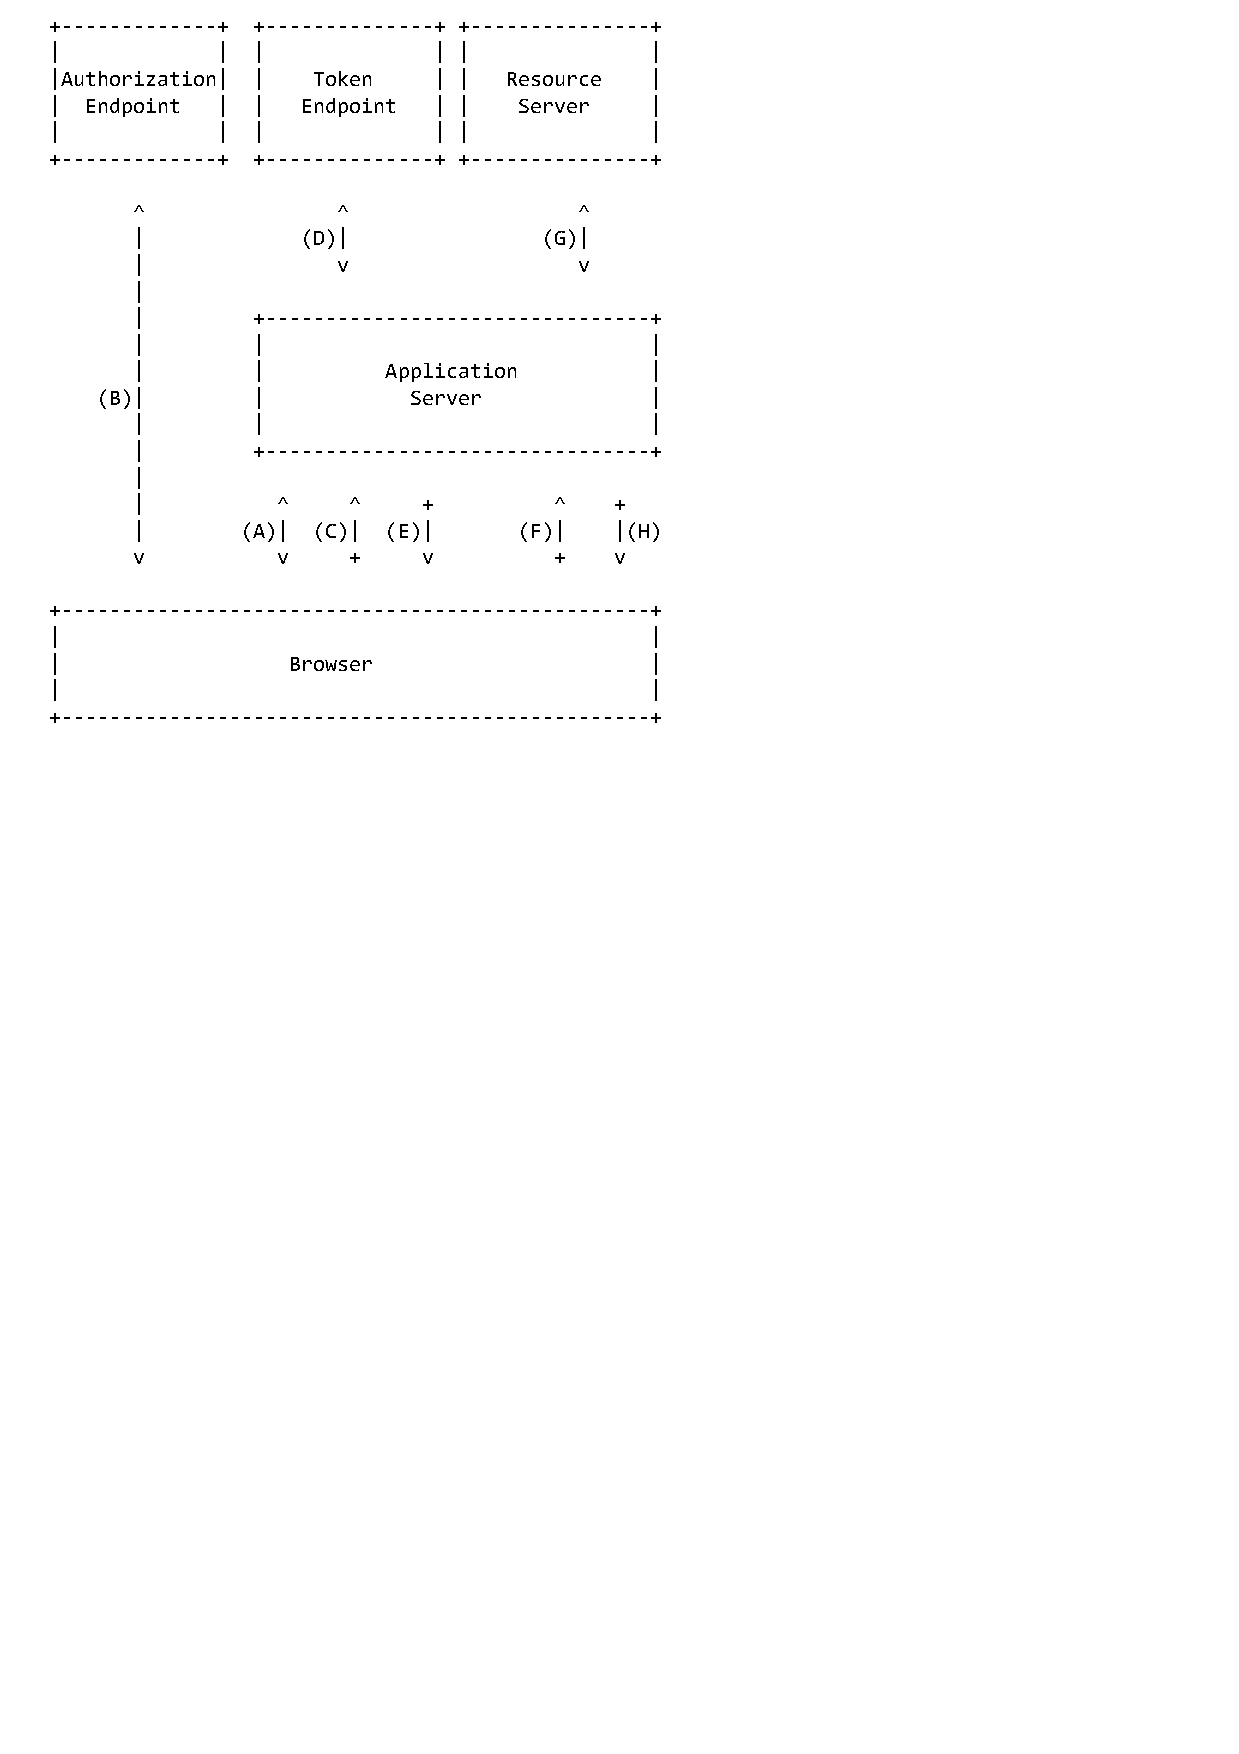
\includegraphics[width=0.7\textwidth]{Graphics/Chapter3/ietf-oauth-draft.pdf}
    \caption{Architecture from an authentication point of view \cite[Section~6.2]{IetfOauthDraft}}
\end{figure}

In our case, the application server is Spring Boot and the authorization endpoint is the Spotify login page (see \autoref{fig:SpotifyLogin}). The token endpoint is a Spotify API endpoint and configured in the Spring Boot application. The only difference to above figure is that the backend application is not setup to serve frontend files (the resource server part). This is because we usually would run the React and Spring Boot application separately during development. Do note that not serving frontend files from the backend application comes with some drawbacks though. For example, we had to disable \ac{CSRF} protection as it does only work if the backend serves frontend files. This brings us to the actual high-level architecture overview from a user perspective.

\begin{figure}[bth]
    \centering
    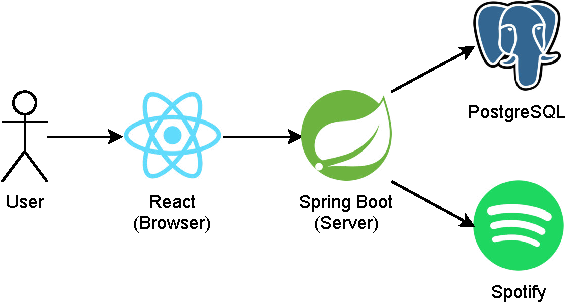
\includegraphics[width=0.8\textwidth]{Graphics/Chapter3/architecture-overview.pdf}
    \caption{Architecture from a user point of view}
\end{figure}

As one can see, the backend application handles communication to the database (PostgreSQL) as well as Spotify (for fetching data and authentication). Frontend and backend exchange data using \ac{HTTP}.

\section{Backend}

\section{Frontend}
